\documentclass{math}

\usepackage{graphicx}
\usepackage{listings}

\title{Intro to Computer Science Theory: Homework 10}
\author{Alvin Lin and Joshua Cotton}
\date{August 2017 - December 2017}

\begin{document}

\maketitle

\subsection*{Problem 1}
\begin{center}
  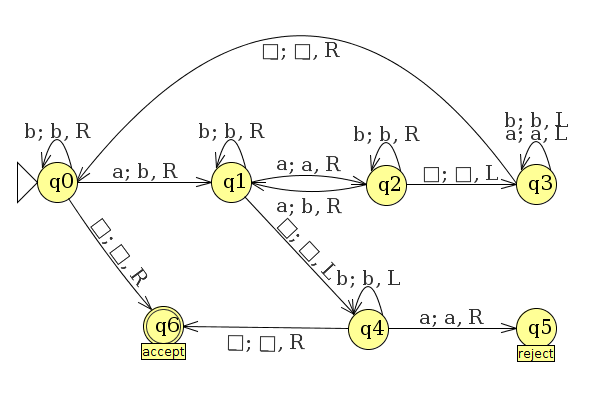
\includegraphics[width=16cm]{assets/hw_10_1.png}
\end{center}
This Turing machine works essentially by taking the length of the input and
``dividing it by 2''. We start from the beginning and cross out every
other \( a \), until we reach the end. If we've reached the end of the string
and the end character was crossed out, then we scan backwards looking for
uncrossed characters. If there were characters that were not crossed out, then
there is a remainder from dividing by two and thus the length is not a power
of 2, otherwise the length is a power of 2 and we accept. If we've reached the
end of the string during the crossing process but the last character was not
crossed out, then we jump back to the start of the string and repeat from the
beginning. For the purpose of the following pseudocode and the diagram above,
we will represent crossed out \( a \)'s as \( b \).
\begin{lstlisting}
Step 1:
  if tape is on the blank character:
    ACCEPT
Step 2:
  while tape is on b:
    move right
  replace a with b
  move right
  if tape is on the blank character:
    go to Step 3
  while tape is on b:
    move right
  if tape is on a:
    move right
  if tape is on the blank character:
    move left back to beginning
    go to Step 1
  go to Step 2
Step 3:
  while tape is on b:
    move left
  if tape is on a:
    REJECT
  if tape is on the blank character:
    ACCEPT
\end{lstlisting}

\begin{center}
  If you have any questions, comments, or concerns, please contact me at
  alvin@omgimanerd.tech
\end{center}

\end{document}
